\section{Uncertainty}
According to \cite{BDA_GCSDVR}, \begin{quote}the central feature of Bayesian inference is the direct quantification of uncertainty.\end{quote}
Bayesian approach to modeling uncertainty is particularly useful when:
\begin{itemize}[noitemsep]
	\item the available data is limited;
	\item there is some concern about overfitting;
	\item some facts are more likely to be true than others, but that information is not contained in the data, or 
	\item the precise likelihood of certain facts is more important than solely determining which fact is most likely (or least likely).
\end{itemize}
The following example represents a Bayesian approach to dealing with the uncertainty of the so-called \textbf{envelope paradox}.
\begin{Example}
You are given two indistinguishable envelopes, each containing a cheque, one being twice as much as the other. You may pick one envelope and keep the money it contains. Having chosen an envelope at will, but before inspecting it, you are given the chance to switch envelopes. Should you switch? What is the expected outcome in doing so? Explain how this game leads to infinite cycling. \newl \textbf{Solution:} let $V$ be the (unknown) value found in the envelope after the first selection. The other envelope then contains either $\frac{1}{2}V$ or $2V$, both with probability $0.5$, and the expected value of trading is $$E[\text{trade}]=0.5\times \frac{1}{2}V + 0.5 \times 2V = \frac{5}{4}V>V;$$ and so it appears that trading is advantageous. Let the (still unknown) value of the cheque in the new envelope be $W$. The same argument shows that the expected value of trading \textit{that} envelope is $\frac{5}{4}W>W$, so it would make sense to trade the envelope once more, and yet once more, and so on, leading to infinite cycling. \newl There is a Bayesian approach to the problem, however. Let $V$ be the (uncertain) value in the original selection, and $W$ be the (also uncertain) value in the second envelope. A proper resolution requires a joint (prior) distribution for $V$ and $W$. Now, in the absence of any other information, the most we can say about this distribution using the maximum entropy principle is that $P(V<W)=P(V>W)=0.5$. \par By definition, if $V<W$, then $W=2V$; if, on the other hand, $V>W$ then $W=\frac{V}{2}$. We now show that the expected value in both envelopes is the same, and thus that trading envelope is no better strategy than keeping the original selection. \newpage\noindent Using Bayes' Theorem, we compute that  
\begin{align*}E[W]&=E[W|V<W]P(V<W) + E[W|V>W]P(V>W) \\ &=E[2V|V<W]\cdot 0.5+E[0.5V|V>W]\cdot 0.5 \\ &= E[V|V<W]+0.25\cdot E[V|V>W],\end{align*} while \begin{align*}E[V]&=E[V|V<W]P(V<W) + E[V|V>W]P(V>W) \\ &=0.5\cdot E[V|V<W]+ 0.5\cdot E[V|V>W].\end{align*}
Before we can proceed any further, we must have some information about the joint distribution $P(V,W)$ (note, however, that $E[W]$ will not typically be equal to $\frac{5}{4}V$, as had been assumed at the start of the solution). \newl 
The domain $\Omega$ of the joint probability consists of those pairs $(V,W)$ satisfying $V=2W$ $(V>W)$ or $W=2V$ ($V<W$) for $0<V,W<M$, where $M<\infty$ is some upper limit on the value of each cheque.\footnote{In the worst case scenario, $M$ would have to be smaller than the total amount of wealth available to humanity throughout history, although in practice $M$ should be substantially smaller. Obviously, a different argument will need to be made in the case $M=\infty$.}
\begin{center}
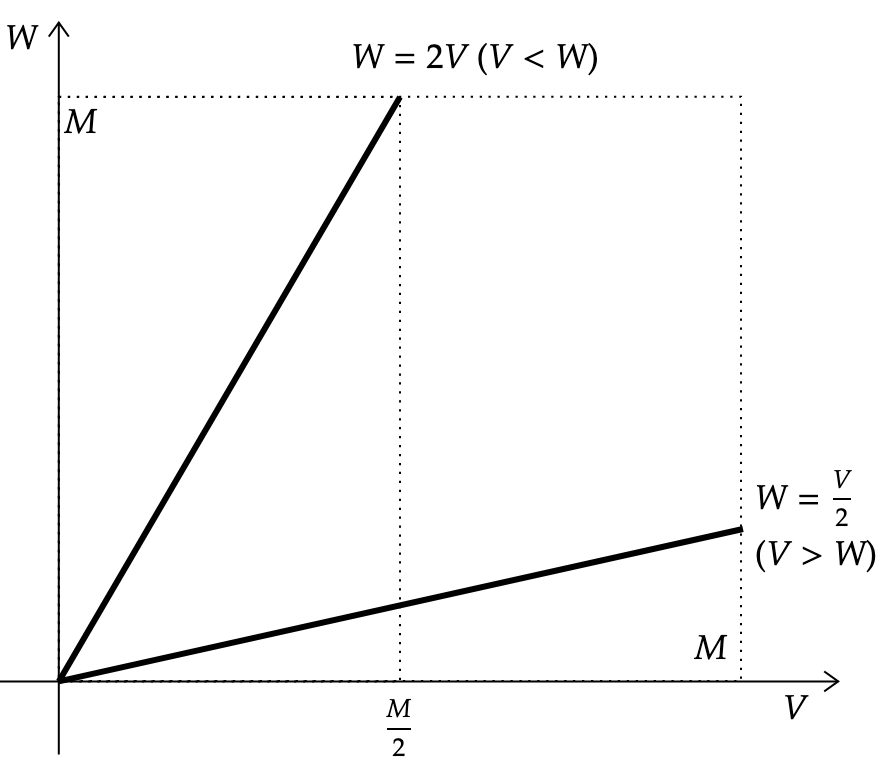
\includegraphics[width=0.9\linewidth]{Images/envelope.png}
\end{center}
\noindent We have assumed that the probability weight on each branch of $\Omega$ is 1/2; if we further assume, say, that the cheque value is as likely to be any of the allowable values on these branches, then the joint distribution is 
$$P(V,W)=\begin{cases}
\frac{1}{M} & \text{if $V<W$} \\
\frac{1}{2M} & \text{if $V>W$} \\
0 & \text{otherwise}
\end{cases}$$
and the expectations listed above are 
$$E[V|V<W]=\int_{V<W}\!\!\!\!\!\!\!\!\!\!\! V\cdot P(V,W)\, d\Omega = \int_{0}^{M/2}\!\!\!\!\!\!\!\!V\cdot\frac{1}{M}\, dV=\frac{M}{8} $$ and $$E[V|V>W]=\int_{V>W}\!\!\!\!\!\!\!\!\!\!\! V\cdot P(V,W)\, d\Omega = \int_{0}^{M}\!\!\!\!V\cdot\frac{1}{2M}\, dV=\frac{M}{4}.$$ Therefore, $$E[W]=\frac{M}{8}+0.25\cdot \frac{M}{4}=\frac{3M}{16}$$ and $$E[V]=0.5\cdot \frac{M}{8}+0.5\cdot \frac{M}{4}=\frac{3M}{16},$$ and switching the envelope does not change the expected value of the outcome. There is no paradox; no infinite cycling.
\end{Example}

\begin{Example} \textit{Bayes in the courtroom.} After the sudden death of her two baby sons, Sally Clark was sentenced by a U.K. court to life in prison in 1996. Among other errors, expert witness Sir Roy Meadow had wrongly interpreted the small probability of two cot deaths as a small probability of Clark's innocence. After a long campaign, which included the refutation of Meadow's statistics using Bayesian statistics, Clark was released in 2003. While Clark's innocence could not be proven beyond the shadow of a doubt using such methods, her culpability could also not be established beyond reasonable doubt and she was cleared. An interesting write-up of the situation can be found online \cite{BDA_NNN}.
\end{Example}

%----------------------------------------------------------------------------------------
%----------------------------------------------------------------------------------------
